\documentclass[]{article}
\usepackage{lmodern}
\usepackage{amssymb,amsmath}
\usepackage{ifxetex,ifluatex}
\usepackage{fixltx2e} % provides \textsubscript
\ifnum 0\ifxetex 1\fi\ifluatex 1\fi=0 % if pdftex
  \usepackage[T1]{fontenc}
  \usepackage[utf8]{inputenc}
\else % if luatex or xelatex
  \ifxetex
    \usepackage{mathspec}
  \else
    \usepackage{fontspec}
  \fi
  \defaultfontfeatures{Ligatures=TeX,Scale=MatchLowercase}
\fi
% use upquote if available, for straight quotes in verbatim environments
\IfFileExists{upquote.sty}{\usepackage{upquote}}{}
% use microtype if available
\IfFileExists{microtype.sty}{%
\usepackage{microtype}
\UseMicrotypeSet[protrusion]{basicmath} % disable protrusion for tt fonts
}{}
\usepackage[margin=1in]{geometry}
\usepackage{hyperref}
\hypersetup{unicode=true,
            pdftitle={Simulation study of efficiency of STM methods},
            pdfauthor={Alan Yang},
            pdfborder={0 0 0},
            breaklinks=true}
\urlstyle{same}  % don't use monospace font for urls
\usepackage{graphicx,grffile}
\makeatletter
\def\maxwidth{\ifdim\Gin@nat@width>\linewidth\linewidth\else\Gin@nat@width\fi}
\def\maxheight{\ifdim\Gin@nat@height>\textheight\textheight\else\Gin@nat@height\fi}
\makeatother
% Scale images if necessary, so that they will not overflow the page
% margins by default, and it is still possible to overwrite the defaults
% using explicit options in \includegraphics[width, height, ...]{}
\setkeys{Gin}{width=\maxwidth,height=\maxheight,keepaspectratio}
\IfFileExists{parskip.sty}{%
\usepackage{parskip}
}{% else
\setlength{\parindent}{0pt}
\setlength{\parskip}{6pt plus 2pt minus 1pt}
}
\setlength{\emergencystretch}{3em}  % prevent overfull lines
\providecommand{\tightlist}{%
  \setlength{\itemsep}{0pt}\setlength{\parskip}{0pt}}
\setcounter{secnumdepth}{0}
% Redefines (sub)paragraphs to behave more like sections
\ifx\paragraph\undefined\else
\let\oldparagraph\paragraph
\renewcommand{\paragraph}[1]{\oldparagraph{#1}\mbox{}}
\fi
\ifx\subparagraph\undefined\else
\let\oldsubparagraph\subparagraph
\renewcommand{\subparagraph}[1]{\oldsubparagraph{#1}\mbox{}}
\fi

%%% Use protect on footnotes to avoid problems with footnotes in titles
\let\rmarkdownfootnote\footnote%
\def\footnote{\protect\rmarkdownfootnote}

%%% Change title format to be more compact
\usepackage{titling}

% Create subtitle command for use in maketitle
\providecommand{\subtitle}[1]{
  \posttitle{
    \begin{center}\large#1\end{center}
    }
}

\setlength{\droptitle}{-2em}

  \title{Simulation study of efficiency of STM methods}
    \pretitle{\vspace{\droptitle}\centering\huge}
  \posttitle{\par}
  \subtitle{Appendix of `Krijkamp EM, Alarid-Escudero F, Enns EA, Hunink MGM,
Pechlivanoglou P, Yang, A., Jalal HJ.' \textbf{A multidimensional array
representation of state-transition model} (revised, September 2019)}
  \author{Alan Yang}
    \preauthor{\centering\large\emph}
  \postauthor{\par}
      \predate{\centering\large\emph}
  \postdate{\par}
    \date{9/26/2019}


\begin{document}
\maketitle

\textbf{Explanation of the simulation study}

We conducted a simulation study on computation efficiency of the two
methods using the \texttt{R} software. The computation time in seconds
and the computation storage in megabytes (MB) of the two methods were
compared. The parameters that were varied were the number of states and
the number of cycles in our cohort model. The number of states varied
from 2 to 62, incremented by 5, while the number of cycles varied from
12 to 1320, incremented by 12. The minimum number of states in a cohort
model is 2 and a cohort model with more than 60 states is not very
common, and should there be more than 60 states alternative approaches
such as microsimulation models are often used instead. The number of
months in 110 years (modelling an individual's lifetime) is 1320, and an
increment of 12 cycles represents annual incrementation.

In order to capture and calculate transition and state rewards using the
cohort trace approach, temporary states had to be created, since the
transition reward for a state is only obtained when it is first visited.
Without loss of generality, we assume there are no absorbing states and
every state can be visited from any other state. Also, the transition
probability matrices for both approaches were randomly sampled such that
each entry is between 0 and 1 and each row adds up to 1. The rewards
vectors and matrices for both approaches were also randomly sampled from
appropriate distributions. We set the seed of \texttt{R}'s random number
generator to assure reproducible results.

At 1320 cycles, as the number of states increases, the run time of the
cohort trace approach increases almost exponentially while that of the
array approach stays invariant, and significantly less. Looking at the
three-dimensional figure that illustrates how computation time of the
two approaches vary as the number of health states and the number of
cycles increase simultaneously. The figure shows that the run time of
the cohort trace approach increases when either the number of health
states or the number of cycles increases. On the contrary, the run time
of the array approach is significantly less and is invariant to
increases in either the number of health states nor the number of
cycles.

At 1320 cycles, as the number of health states increases, the storage of
both approaches increases. When the number of health states is less than
approximately 52, the cohort trace approach takes up less storage. But
when the number of health states is above approximately 52, it takes up
more storage. Looking at the three-dimensional figure that illustrates
how computation storage of the two approaches vary as the number of
health states and the number of cycles increase simultaneously. We see
that the storage increases as when either the number of health states or
the number of cycles increases. Both approaches take up approximately
the same amount of storage before around 50 health states. After 50
health states the cohort trace approach takes up more memory compared to
the array approach.

Based on the results of our simulation study, we conclude that the array
approach is computationally superior to the cohort trace approach. It is
much faster and does not run any slower when the number of cycles or the
number of health states increases. In addition, it takes up less storage
as the number of states becomes sufficiently large. All code of the
simulation study and to make the figures can be found on

\textbf{Compare time:}

2D line graph - by state, at 1320 cycles

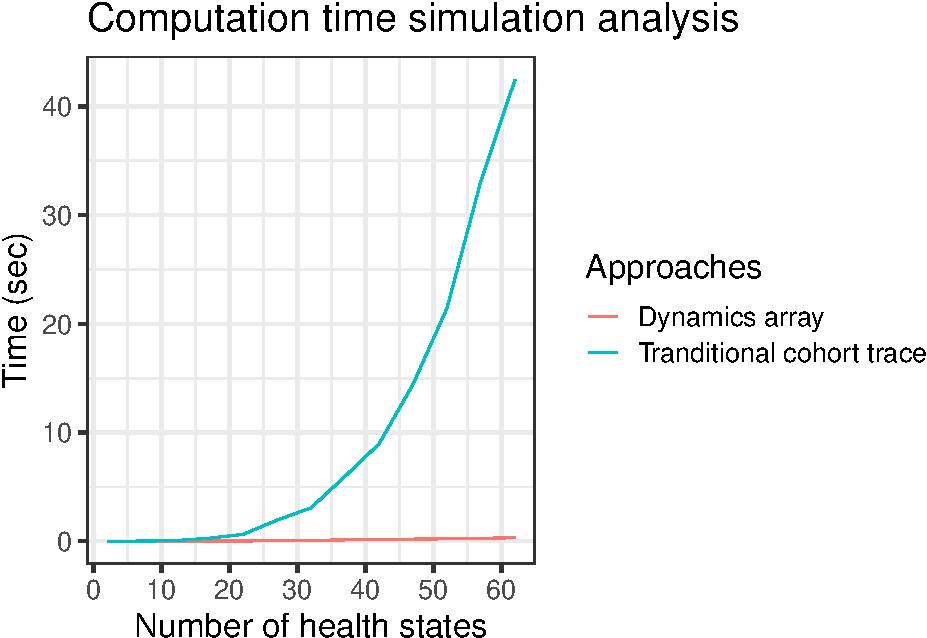
\includegraphics{compare_time_memory_files/figure-latex/unnamed-chunk-1-1.pdf}

\textbf{Zoom in on the y-axis}

2D line graph - by state, at 1320 cycles zoomed in on the y-axis to see
time changes of the array approach
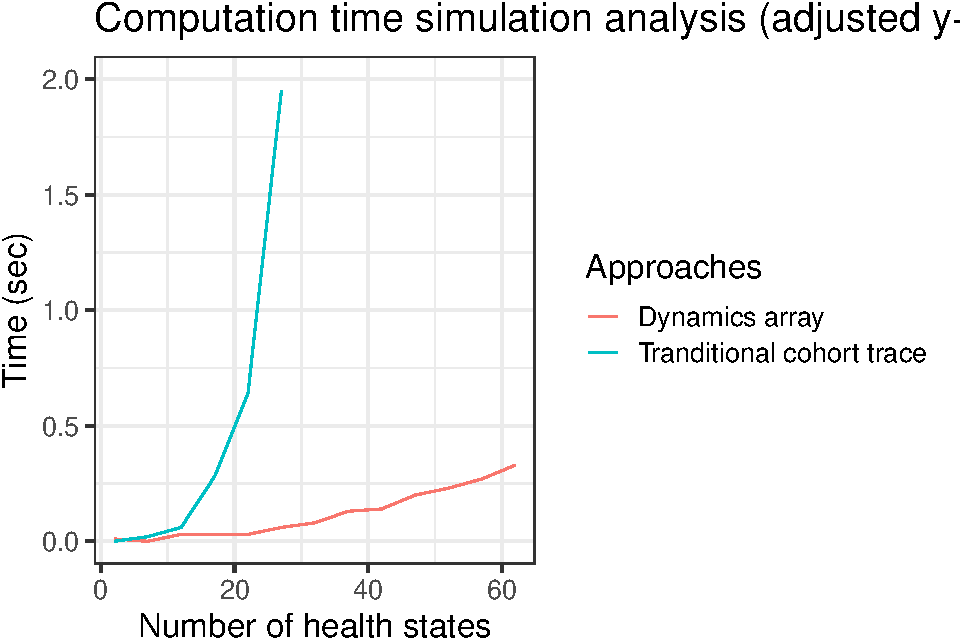
\includegraphics{compare_time_memory_files/figure-latex/unnamed-chunk-2-1.pdf}

3D Scatter plot:

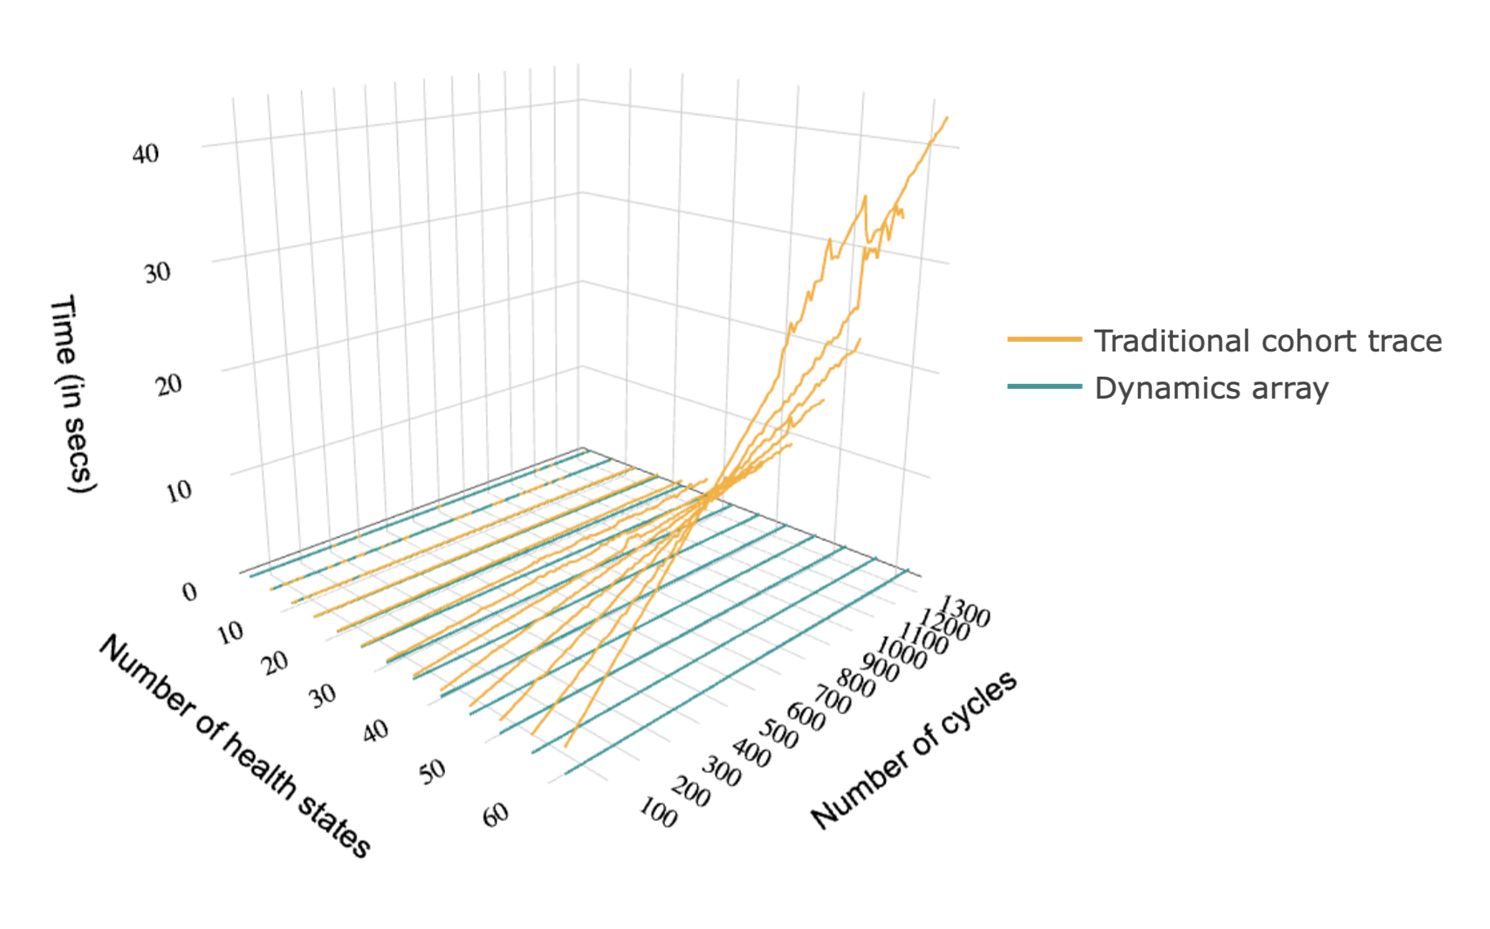
\includegraphics[width=1\linewidth]{3D_time}

\textbf{Compare storage:}

2D line graph - by state, at 1320 cycles

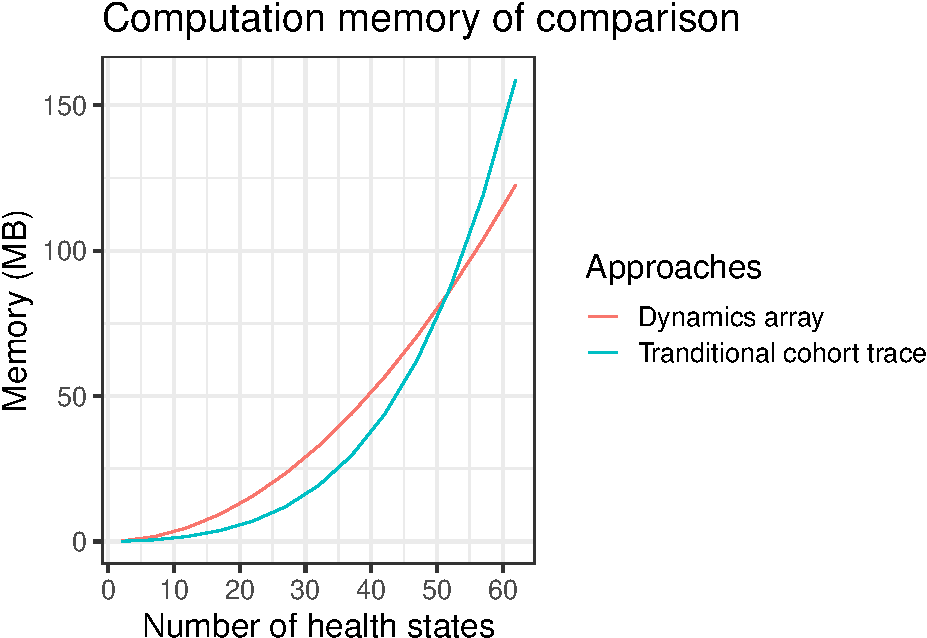
\includegraphics{compare_time_memory_files/figure-latex/unnamed-chunk-5-1.pdf}

3D Scatter plot:

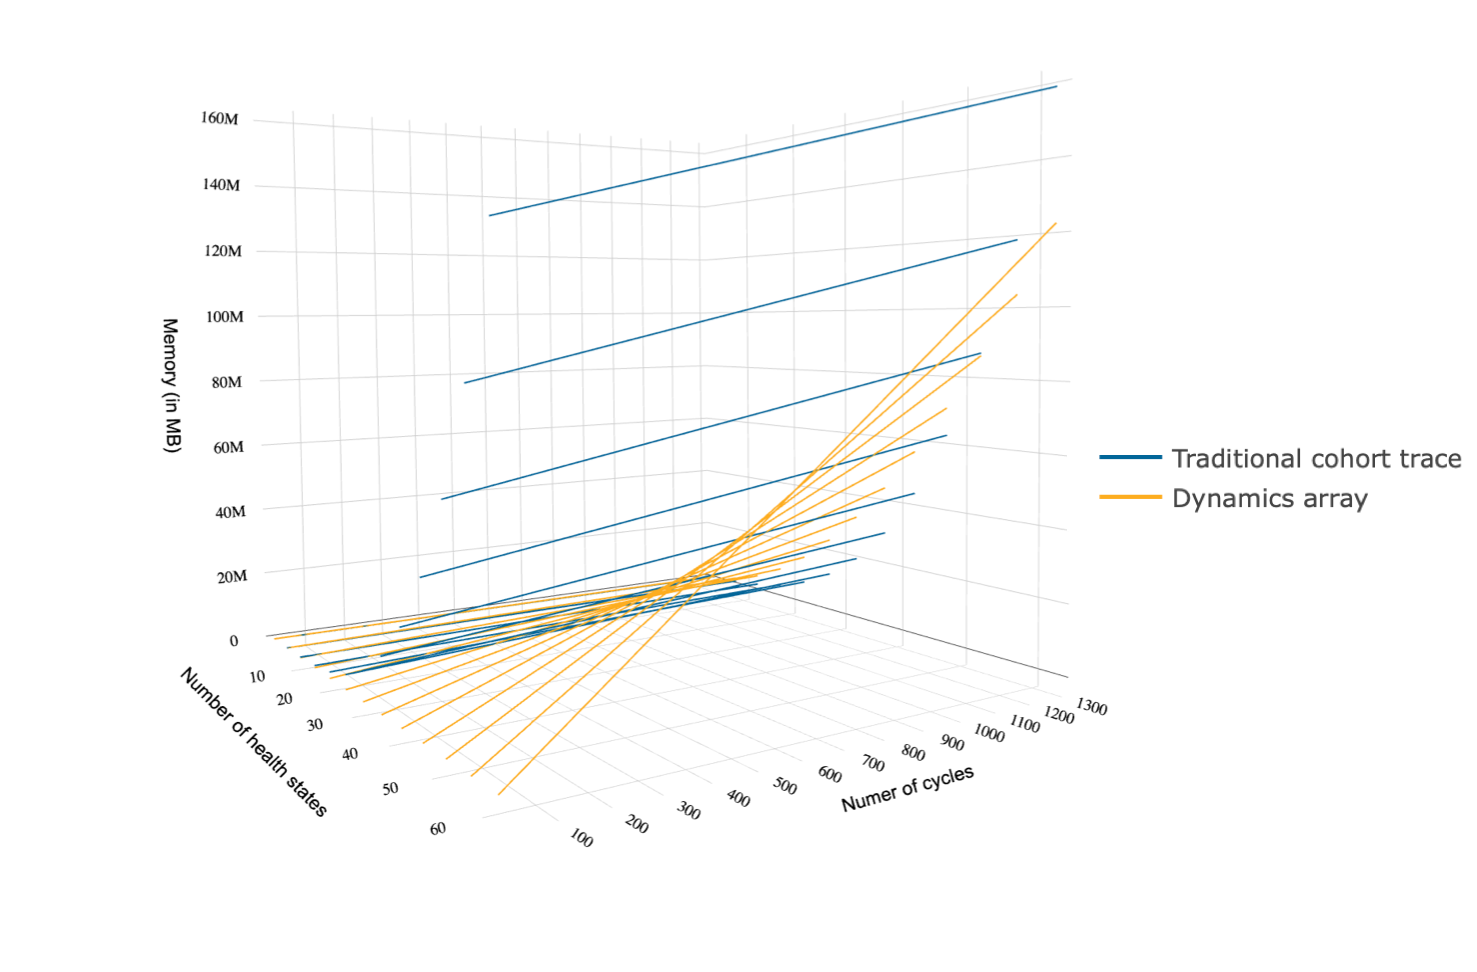
\includegraphics[width=1\linewidth]{3D_memory}


\end{document}
